\documentclass[a4paper]{article}
\usepackage[utf8]{inputenc}
\usepackage[russian,english]{babel}
\usepackage[T2A]{fontenc}
\usepackage[left=10mm, top=20mm, right=18mm, bottom=15mm, footskip=10mm]{geometry}
\usepackage{indentfirst}
\usepackage{amsmath,amssymb}
\usepackage{mathastext} 
\usepackage[italicdiff]{physics}
\usepackage{graphicx}
\usepackage{caption}
\usepackage{float}
\usepackage{caption}
\renewcommand{\thefootnote}{\fnsymbol{footnote}}
\usepackage{tablefootnote}
\usepackage{footmisc}
\usepackage{textcomp}
\usepackage{multicol}
\usepackage[parfill]{parskip}
\usepackage{makecell}
\usepackage{array}  
\renewcommand\cellalign{cc} 
\renewcommand\cellgape{\Gape[2pt]} 
\usepackage[utf8]{inputenc}\newcommand{\approxtext}[1]{\ensuremath{\stackrel{\text{#1}}{\approx}}}
\usepackage[colorlinks=true, urlcolor=blue, linkcolor=blue, citecolor=blue]{hyperref}
\graphicspath{{images/}}
\DeclareGraphicsExtensions{.pdf,.png,.jpg}
\usepackage{wrapfig}
\captionsetup{labelformat=empty}
\usepackage{caption}
\captionsetup[figure]{name=Рисунок}
\captionsetup[table]{name=Таблица}
  
\title{\textbf{Отчет о выполнении лабораторной работы 3.4.5}}
\date{}
\author{Котляров Михаил, Б01-402}

\begin{document}

\maketitle
	
	\section{Введение}
	
	\textbf{Цель работы:} изучение петель гистерезиса различных ферромагнитных материалов в переменных полях;\\

	\textbf{Оборудование:} автотрансформатор, понижающий трансформатор, интегрирующая ячейка, амперметр и вольтметр, резистор, делитель напряжения, электронный осциллограф, тороидальные образцы с двумя обмотками.
	
	\section{Теоретические сведения}

\subsection*{Магнитное поле в веществе и его микроскопическая природа}

Вещество может обладать как собственной намагниченностью, так и изменять свою намагниченность под действием внешнего магнитного поля. Микроскопическими источниками магнитного поля в среде являются орбитальное движение электронов в атомах и молекулах, а также их собственный спин. В рамках классического подхода каждый элемент объёма вещества можно рассматривать как магнитный диполь, обладающий магнитным моментом. Для описания усреднённых макроскопических свойств среды вводится \textbf{вектор намагниченности} $\vec{J}$, равный магнитному моменту единичного объёма вещества.

Магнитное поле в веществе характеризуется двумя основными векторами: \textbf{магнитной индукцией} $\vec{B}$ и \textbf{напряжённостью магнитного поля} $\vec{H}$. Величина $\vec{B}$ — это полная магнитная индукция, измеряемая в теслах (Тл), и она определяется как предел отношения суммарного магнитного потока через малый объём к его объёму:
\begin{equation}
\vec{B} = \lim_{\Delta V \to 0} \frac{\sum \vec{B}_{\text{микро}}}{\Delta V}.
\end{equation}
Вектор $\vec{H}$ вводится как вспомогательная величина, связанная с токами проводимости, и определяется соотношением:
\begin{equation}
\vec{B} = \mu_0 (\vec{H} + \vec{M}),
\end{equation}
где $\mu_0 = 4\pi \cdot 10^{-7}$~Гн/м — магнитная постоянная. Отсюда следует, что $\vec{H}$ зависит только от свободных токов, тогда как $\vec{B}$ учитывает как свободные, так и связанные (индукционные) токи.

В простейшем случае намагниченность пропорциональна напряжённости поля:
\begin{equation}
\vec{M} = \chi \vec{H},
\end{equation}
где $\chi$ — \textbf{магнитная восприимчивость}, безразмерная величина, характеризующая реакцию вещества на внешнее поле. Тогда:
\begin{equation}
\vec{B} = \mu_0 (1 + \chi)\vec{H} = \mu_0 \mu \vec{H},
\end{equation}
где $\mu = 1 + \chi$ — относительная магнитная проницаемость. Заметим, что это линейное соотношение справедливо лишь для диа- и парамагнетиков; в ферромагнетиках зависимость $\vec{M}(\vec{H})$ нелинейна и сопровождается гистерезисом.

\subsection*{Диамагнетизм}

Диамагнетизм ($\chi < 0$) — универсальное явление, присущее всем веществам, но проявляющееся наиболее ярко у веществ, не имеющих собственных магнитных моментов (например, Bi, Cu). Природа диамагнетизма — электромагнитная индукция: при включении внешнего магнитного поля $\vec{B}$ в атомах возникают индуцированные токи , которые создают магнитный момент, направленный против поля.

\begin{equation}
\chi_{\text{диа}} \sim -\mu_0 \frac{e^2 a^2 Z n}{4 m_e},
\end{equation}
где $a$ — среднее расстояние между электронами и ядром, $Z$ — заряд ядра, $n$ — плотность атомов. Диамагнитная восприимчивость не зависит от температуры и имеет порядок $10^{-6}$, что делает её слабым эффектом.

\subsection*{Парамагнетизм}

Парамагнетики ($\chi > 0$) — вещества, содержащие атомы или ионы с собственным магнитным моментом (например, O$_2$, Al). В отсутствие внешнего поля эти моменты ориентированы хаотично из-за теплового движения, поэтому средняя намагниченность равна нулю. При включении поля $\vec{H}$ происходит преимущественная ориентация моментов по полю, что приводит к положительной намагниченности.

Сила, действующая на магнитный момент $\vec{m}$ в неоднородном поле, стремится выстроить его по направлению $\vec{B}$. Однако тепловое движение препятствует полной ориентации. В классической модели средний момент направлен по полю, и восприимчивость оказывается обратно пропорциональной температуре (закон Кюри):
\begin{equation}
\chi \propto \frac{1}{T}.
\end{equation}
Парамагнетизм характеризуется малой восприимчивостью ($\chi \sim 10^{-3} - 10^{-5}$) и отсутствием гистерезиса.

\subsection*{Ферромагнетизм}

Помимо диа- и парамагнетиков, в природе существуют вещества, способные сильно намагничиваться даже в небольших полях. Такие вещества относят к классу \textbf{ферромагнетиков}. Это — железо, никель, кобальт, гадолиний и их многочисленные сплавы. Ферромагнитными свойствами обладают некоторые сплавы элементов, которые порознь не являются ферромагнитными (например, сплавы меди и марганца), и ряд неметаллических веществ (ферриты). Ферромагнитные явления сложны и многообразны, и мы ограничимся изложением лишь некоторых основных фактов.

Зависимость намагниченности $M$ от напряжённости магнитного поля $H$ у всех ферромагнетиков оказывается \textbf{нелинейной}: магнитная восприимчивость $\chi$ не является константой и зависит от $H$.

Как и в случае парамагнетиков, атомы ферромагнетика обладают собственным магнитным моментом. Однако даже в отсутствие внешнего магнитного поля атомы ферромагнетика способны образовывать упорядоченные структуры (\textbf{домены}), в которых все магнитные моменты ориентированы практически в одном направлении. Таким образом, каждый отдельный атом испытывает влияние не только внешнего поля, но и поля, созданного коллективом его соседей.

\subsection*{Образование доменов}
Остановимся кратко на причине, по которой соседним магнитным моментам выгодно объединяться в домены. В первую очередь подчеркнём, что магнитное (диполь-дипольное) взаимодействие между атомами не может привести к упорядочению системы, т.к. тепловое движение обеспечит полное разупорядочение уже при $T \sim 1$~К.

Единственное взаимодействие, которое способно выстроить в ряд магнитные моменты электронов в атомах при температурах порядка комнатной, — это \textbf{электростатическое взаимодействие} (его энергия на несколько порядков больше магнитной: $e^2/(4\pi\varepsilon_0 a) \sim 1$~эВ). Как следует из квантовой механики, если магнитные моменты (или спины) электронов соседних атомов сонаправлены, их электростатическая отталкивание становится меньше. Таким образом, магнитным моментам атомов энергетически выгодно ориентироваться в одном направлении. Такое явление получило название \textbf{обменного взаимодействия}.

С другой стороны, магнитное диполь-дипольное взаимодействие между доменами препятствует выстраиванию всех магнитных моментов среды в одном направлении. Действительно, энергия такого взаимодействия будет минимальной при антитпараллельном расположении магнитных моментов соседних элементов среды. Поэтому при определённом поперечном размере домена оказывается энергетически выгодно иметь соединённый домен с противоположно ориентированным моментом.

Наложение внешнего поля заставляет домены ориентироваться по нему, что приводит к резкому увеличению намагниченности образца, а при достаточно большом поле достигается состояние \textbf{насыщения}, когда все домены ориентируются по полю.

\subsection*{Ферромагнитный гистерезис}

Если состояние некоторой системы зависит не только от мгновенных значений внешних параметров, но и от истории их изменений, говорят, что в системе имеет место \textbf{гистерезис}. Именно такими свойствами обладает магнитный момент ферромагнитного образца как функция напряжённости поля $M(H)$. В частности, система может оказаться намагниченной, даже когда внешнее поле выключено — этим объясняется существование постоянных магнитов. 
\textbf{Кривая намагничивания}. Пусть ферромагнетик находится в ненамагниченном состоянии ($M = 0$). Медленно увеличивая поле $H$ в образце, получим зависимость $M(H)$, которую называют \textbf{начальной кривой намагничивания}. Эту кривую обычно разделяют на пять условных участков (рис. 1).

\begin{figure}[h]
        \center{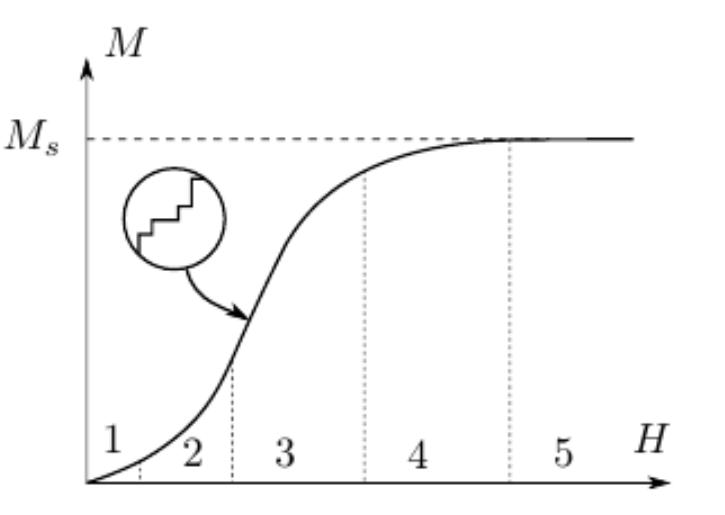
\includegraphics[width=0.5\textwidth]{Pictures/magnetic_curve.png}}
        \caption{Рис 1. Начальная кривая намагничивания ферромагнетика.}
\end{figure}

Участок 1 — область \textbf{обратимого намагничивания}, где $M = \chi H$. В этой области происходят процессы упругого смещения границ доменов: увеличивается размер тех доменов, магнитный момент которых близок к направлению магнитного поля, и уменьшаются размеры доменов с противоположным направлением магнитного момента.

Участок 2 характеризуется квадратичной зависимостью $M$ от $H$. В этой области также идёт процесс обратимого смещения границ, но проявляется нелинейный характер зависимости намагниченности от поля.

Область максимальной скорости роста намагниченности 3 соответствует \textbf{необратимым смещениям стенок между доменами}: им приходится преодолевать «препятствия» в виде примесей, дислокаций и дефектов кристаллической решётки. Когда стенка наталкивается на такое препятствие, она останавливается и держится, пока поле не достигнет порогового значения, при котором она внезапно срывается. Таким образом, движение доменной стенки приобретает скачкообразный характер.

В достаточно сильных полях движение стенок прекращается, и энергетически выгодным становится поворот магнитных моментов тех оставшихся доменов, у которых магнитный момент не совпадает с направлением поля (область 4).

И, наконец, при некотором значении поля (участок 5) все магнитные моменты выстраиваются по полю — намагниченность достигает \textbf{насыщения} ($M = M_s$).

Наклон кривой намагничивания характеризуется \textbf{дифференциальной магнитной проницаемостью}:
\begin{equation}
\mu_{\mathrm{диф}} = \frac{1}{\mu_0} \frac{dB}{dH}.
\end{equation}
С ростом $H$ величина $\mu_{\mathrm{диф}}$ сначала растёт (этому соответствуют участки 1 и 2 на рис. 1), затем (с середины участка 3) начинает резко падать, приближаясь к единице при насыщении.

\begin{figure}[h]
        \center{
\includegraphics[width=0.5\textwidth]{Pictures/1.png}}
        \caption{Рис 2. Начальная кривая намагничивания и предельная петля гистерезиса}
\end{figure}
\textbf{Явление гистерезиса}. Доведём систему до некоторой точки $A$, лежащей в области насыщения (здесь $B_s$ — \textbf{индукция насыщения}), и начнём уменьшать напряжённость $H$. Поскольку между доменами есть трение, обратный путь пойдёт не по начальной кривой, а \textit{иначе}.

При выключении внешнего поля, то есть при достижении $H = 0$, в образце сохраняется некоторое собственное намагничивание. Соответствующее значение индукции $B_r$ называют \textbf{остаточной индукцией}.

Значение $B = 0$ достигается лишь при некотором отрицательном значении $H = -H_c$. Величина $H_c$ называется \textbf{коэрцитивным полем}. Среди ферромагнетиков принято различать \textbf{магнитомягкие} ($H_c \lesssim 1$~кА/м) и \textbf{магнитотвёрдые} ($H_c > 10$~кА/м) материалы. В точке $C$ наступает насыщение для намагничивания в противоположную сторону.

Если теперь попробовать вернуться в точку $A$, вновь наращивая поле, получим повторный замкнутый цикл (предельную петлю) — \textbf{петлю гистерезиса}. Если в точке $A$ насыщение не достигается, то аналогичным образом получится цикл меньшей площади.

Отметим, что площадь петли гистерезиса ферромагнетика на плоскости $H$--$B$ есть энергия, \textbf{необратимо} выделяющаяся в виде тепла в единице объёма вещества за один цикл:
\begin{equation}
\Delta w = -\oint H dB
\end{equation}

\subsection*{Измерение магнитной индукции}

Магнитную индукцию $B$ удобно определять с помощью ЭДС, возникающей при изменении магнитного потока $\Phi$ в катушке, намотанной на образец. Пусть катушка с $N$ витками имеет охватываемое сечением $S$ и индукция $B$ в образце однородна. Имеем:
\begin{equation}
|B| = \frac{1}{SN} \int \varepsilon dt.
\end{equation}

Таким образом, для определения $B$ нужно проинтегрировать сигнал, наведённый меняющимся магнитным полем в измерительной катушке, намотанной на образец.

Для интегрирования в работе используется \textbf{интегрирующая $RC$-цепочка} (рис. 3). «Входное» напряжение от источника $U_{\mathrm{вх}}(t)$ подаётся на последовательно соединённые резистор $R_{\text{и}}$ и конденсатор $C_{\text{и}}$. «Выходное» напряжение $U_{\mathrm{вых}}(t)$ снимается с конденсатора.

\begin{figure}[h]
        \center{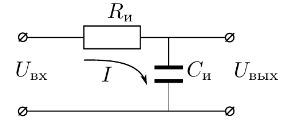
\includegraphics[width=0.3\textwidth]{Pictures/Int_chain.png}}
        \caption{Рис 3. Начальная кривая намагничивания и предельная петля гистерезиса}
\end{figure}

Предположим, что 1) сопротивление источника мало по сравнению с $R_{\text{и}}$, 2) выходное сопротивление (сопротивление на входе осциллографа), напротив, велико: $R_{\mathrm{вых}} \gg R_{\text{и}}$, и, наконец, 3) сопротивление $R_{\text{и}}$ достаточно велико, так что $U_{\mathrm{вых}} \ll U_{\mathrm{вх}}$. В таком случае ток цепи равен $I = (U_{\mathrm{вх}} - U_{\mathrm{вых}})/R_{\text{и}} \approx U_{\mathrm{вх}}/R_{\text{и}}$, и входное и выходное напряжения связаны соотношением:
\begin{equation}
U_{\mathrm{вых}} = \frac{q}{C_{\text{и}}} = \frac{1}{C_{\text{и}}} \int_0^t I dt \approx \frac{1}{\tau_{\text{и}}} \int_0^t U_{\mathrm{вх}} dt,
\end{equation}
где $\tau_{\text{и}} = R_{\text{и}} C_{\text{и}}$ — постоянная времени $RC$-цепочки. Для индукции поля из (9) получаем:
\begin{equation}
|B| = \frac{1}{SN} \left| \int U_{\mathrm{вх}} dt \right| = \frac{\tau_{\text{и}}}{SN} U_{\mathrm{вых}},
\end{equation}

\section*{Экспериментальная установка}

Схема установки изображена на рис.~4. Напряжение сети (220~В, 50~Гц) с помощью трансформаторного блока $T$, состоящего из регулировочного автотрансформатора и разделительного понижающего трансформатора, подаётся на намагничивающую обмотку $N_0$ исследуемого образца.
\begin{figure}[h]
        \center{
\includegraphics[width=0.7\textwidth]{Pictures/ustanovka.png}}
        \caption{Рис 3. Схема установки}
\end{figure}
В цепь намагничивающей катушки, на которую подаётся некоторое напряжение $U_0$, последовательно включено сопротивление $R_0$. Напряжение на $R_0$, равное $U_R = R_0 I_0$, где $I_0$ — ток в намагничивающей обмотке $N_0$, подаётся на канал $X$ осциллографа. Связь напряжённости $H$ в образце и тока $I_0$ рассчитывается по теореме о циркуляции.

Действующее значение переменного тока в обмотке $N_0$ измеряется амперметром $A$.

Для измерения магнитной индукции $B$ в измерительной обмотке $N_{\text{и}}$ на вход интегрирующей ячейки подаётся напряжение $U_{\mathrm{вх}}(U_{\mathrm{вх}})$, пропорциональное производной $dB/dt$. С интегрирующей ячейки $C_{\text{и}}$ снимается напряжение $U_C(U_{\mathrm{вых}})$, пропорциональное величине $B$, и подаётся на канал $Y$ осциллографа. Значение индукции поля $B$ рассчитывается по формуле (11).

Замкнутая кривая, возникающая на экране, воспроизводит в некотором масштабе (различном для осей $X$ и $Y$) петлю гистерезиса. Чтобы придать этой кривой количественный смысл, необходимо установить масштабы изображения, т.~е. провести калибровку каналов $X$ и $Y$ осциллографа.


\section{Выполнение}
\begin{enumerate}

\subsection{Алгоритм действий.}
\item Соберем схему согласно рис. 3. и включим ее в сеть.

\item С помощью источника питания подберем ток в намагничивающей обмотке так, чтобы на экране наблюдалась предельная петля гистерезиса. 

\item Подберем коэффициенты усиления каналов ЭО (электронного осциллографа) так, чтобы предельная петля занимала большую часть экрана. Проведем центрировку вертикального и горизонтального лучей. Сфотографируем предельную петлю. Зафиксируем параметры тороида, значения коэффициентов усиления $K_X$ и $K_Y$.

\item По экрану ЭО измерим полную ширину и высоту предельной петли ($2X_s$ и $2Y_s$), соответствующие удвоенной амплитуде колебания напряженности $H_s$ и индукции $B_s$ поля в образце в состоянии насыщения.

\item Измерим двойные амплитуды для коэрцитивного поля $[2X_c]$ и остаточной индукции $[2Y_c]$. Запишем соответствующие значения коэффициентов усиления $K_X$ и $K_Y$.

\item Плавно уменьшая ток намагничивания от насыщения до нуля, будем отмечать вершины наблюдаемых петель.

\item Рассчитаем цену деления петли в $\frac{A/\text{м}}{\text{дел}}$ для оси $X$ по формуле $H = \frac{K_X N_0}{2\pi R R_0}$; и в $\frac{\text{Тл}}{\text{дел}}$ для оси $Y$ по формуле $B = \frac{\tau_{\text{и}}K_Y}{S N_{\text{и}}}$, где $\tau_{\text{и}} = R_{\text{и}}C_{\text{и}}$, $S$, $N_{\text{и}}$, $R_0$, $N_0$ указаны на установке.

\item Проверка калибровки канала $X$ ЭО

Проведём проверку калибровки канала $X$ электронного осциллографа (ЭО) с помощью амперметра. Для этого:

\begin{enumerate}
    \item Закоротим обмотку $N_0$ образца, так как катушка с ферромагнитным сердечником является нелинейным элементом, и ток в ней не имеет синусоидальной формы. Поэтому связь между амплитудой тока и показаниями амперметра будет очень неточной при наличии образца.
    
    \item Подадим переменное напряжение на обмотку $N_0$, но поскольку она закорочена, ток в цепи станет синусоидальным, и его можно измерить точно.
    
    \item Измерим эффективное значение тока $I_{\mathrm{эф}}$ с помощью амперметра $A$, включённого последовательно с сопротивлением $R_0$.
    
    \item Снимем сигнал с сопротивления $R_0$ и подадим его на вход $X$ ЭО. Это напряжение пропорционально току: $U = I R_0$.
    
    \item На экране ЭО появится горизонтальная прямая, ширина которой соответствует удвоенной амплитуде напряжения на $R_0$.
    
    \item Измерим длину этой прямой $2x$ в делениях экрана.
    
    \item Рассчитаем чувствительность канала $X$ по формуле:
    \[
    K_X = \frac{2 R_0 \sqrt{2} I_{\mathrm{эф}}}{2x} \quad [\text{В/дел}].
    \]
    
    \item Сравним полученное значение $K_X$ с выбранным коэффициентом усиления канала $X$ на панели управления ЭО.
    
    \item Оценим погрешность измерений.
\end{enumerate}

\item Проверка калибровки канала $Y$ ЭО

Проведём проверку калибровки канала $Y$ ЭО с помощью вольтметра. Для этого:

\begin{enumerate}
    \item Отключим тороид, так как несинусоидальный ток нагрузки в первичной обмотке тороида искажает форму напряжения на вторичной обмотке, питающей делитель.
    
    \item Подадим сигнал с обмотки 12,6~В понижающего трансформатора на делитель напряжения.
    
    \item Снимем часть этого напряжения с делителя с коэффициентом деления $K_{\mathrm{д}} = 1/10$ или $1/100$ и подадим на вход $Y$ ЭО.
    
    \item Подключим мультиметр $V$ к тем же клеммам делителя и измерим эффективное напряжение $U_{\mathrm{эф}}$.
    
    \item На экране ЭО появится вертикальная прямая. Измерим её длину $2y$ в делениях.
    
    \item Рассчитаем чувствительность канала $Y$ по формуле:
    \[
    K_Y = \frac{2\sqrt{2} U_{\mathrm{эф}}}{2y} \quad [\text{В/дел}].
    \]
    
    \item Сравним полученное значение $K_Y$ с выбранным коэффициентом усиления канала $Y$.
    
    \item Оценим погрешности измерения амплитуд с помощью ЭО.
    
    \item Повторим проверку для всех значений $K_X$ и $K_Y$, которые использовались в работе.

\item Повторим данный алгоритм для 3-х тороидов.
\end{enumerate}
\subsection{Полученные данные}

\item Параметры тороидов и установки

\begin{table}[h!]
    \centering
    \begin{tabular}{|l|c|c|c|c|}
        \hline
        Материал & $N_0$ & $N_u$ & $S,\ \text{см}^2$ & $2\pi R,\ \text{см}$ \\ \hline
        Пермаллой нп50 & 40 & 200 & 3{,}8 & 24 \\ \hline
        Феррит нн1000 & 35 & 400 & 3 & 25 \\ \hline
        Кремнистое железо & 40 & 400 & 1{,}2 & 10 \\ \hline
    \end{tabular}
    \caption{Таблица 1. Параметры образцов: число витков, площадь сечения и длина средней линии.}
    \label{tab:geometry_params}
\end{table}

\begin{table}[h!]
    \centering
    \begin{tabular}{|c|c|c|c|}
        \hline
        $R_u,\ \text{кОм}$ & $C_u,\ \text{мкФ}$ & $R_0,\ \text{Ом}$ & $\tau,\ \text{Ом}\cdot\text{Ф}$ \\ \hline
        20 & 20 & 0{,}3 & 0{,}4 \\ \hline
    \end{tabular}
    \caption{Таблица 2. Параметры цепи: сопротивления, ёмкость.}
    \label{tab:circuit_params}
\end{table}

\item Проверка калибровки.

\textbf{Замечание.} $2x$ и $2y$ записаны в мелких делениях, а не в клетках, поэтому нужно учесть и поделить на 5 (5 делений в клетке).
\begin{table}[h!]
    \centering
    \begin{tabular}{|l|c|c|c|}
        \hline
        Параметр & Пермаллой & Феррит & Крем. железо \\ \hline
        $K_X,\ \text{мВ/дел}$ & 50 & 20 & 100 \\ \hline
        $K_Y,\ \text{мВ/дел}$ & 20 & 20 & 50 \\ \hline
        $2x$ & 18 & 40 & 30 \\ \hline
        $2y$ & 26 & 22 & 26 \\ \hline
        $I_{\text{эф}},\ \text{мА}$ & 209 & 192 & 699 \\ \hline
        $U_{\text{эф}},\ \text{мВ}$ & 36{,}7 & 30{,}3 & 90{,}1 \\ \hline
        $K_X^{\text{эксп}},\ \text{мВ/дел}$ & 49{,}262 & 20{,}365 & 98{,}854 \\ \hline
        $K_Y^{\text{эксп}},\ \text{мВ/дел}$ & 19{,}962 & 19{,}478 & 49{,}008 \\ \hline
        $\Delta K_X,\ \text{мВ/дел}$ & 0{,}738 & 0{,}365 & 1{,}146 \\ \hline
        $\Delta K_Y,\ \text{мВ/дел}$ & 0{,}038 & 0{,}522 & 0{,}992 \\ \hline
        $\varepsilon_{K_X},\ \%$ & 1{,}48 & 1{,}82 & 1{,}15 \\ \hline
        $\varepsilon_{K_Y},\ \%$ & 0{,}19 & 2{,}61 & 1{,}98 \\ \hline
    \end{tabular}
    \caption{Таблица 3. Сравнение теоретических и экспериментальных значений коэффициентов усиления осциллографа для трех образцов.}
    \label{tab:oscilloscope_calibration}
\end{table}

Как мы видим, масштаб совпадает с выставленным. В качестве погрешности $X$ и $Y$ будем брать $\sigma = \sqrt{(\Delta K)^2 + (0,5 \text{ дел})^2}$, поскольку систематическая и калибровочная погрешности независимы.

\item Поля $H$ и $B$ на цену деления:
\begin{table}[h!]
    \centering
    \begin{tabular}{|l|c|c|c|c|c|c|}
        \hline
        Материал & $H,\ \frac{\text{А/м}}{\text{дел}}$ & $B,\ \frac{\text{Тл}}{\text{дел}}$ & $\sigma_H,\ \frac{\text{А/м}}{\text{дел}}$ & $\sigma_B,\ \frac{\text{Тл}}{\text{дел}}$ & $\varepsilon_H,\ \%$ & $\varepsilon_B,\ \%$ \\ \hline
        Пермаллой & 27{,}778 & 0{,}105 & 0{,}495 & 0{,}003 & 1{,}78 & 2{,}51 \\ \hline
        Феррит & 9{,}333 & 0{,}067 & 0{,}289 & 0{,}002 & 3{,}09 & 3{,}62 \\ \hline
        Кремнистое железо & 133{,}333 & 0{,}417 & 1{,}668 & 0{,}009 & 1{,}25 & 2{,}22 \\ \hline
    \end{tabular}
    \caption{Таблица 4. Магнитные параметры образцов.}
    \label{tab:magnetic_params}
\end{table}

\item Максимальная ампилтуда напряженности $H_{max}$, соответствующая индукции насыщения $B_s$, коэрцетивное поле $H_c$ и остаточная индукция $B_r$:

\begin{table}[h!]
    \centering
    \begin{tabular}{|l|c|c|c|c|c|c|}
        \hline
        Материал & $H_{\max},\ \text{А/м}$ & $B_s,\ \text{Тл}$ & $2X_c,\ \text{дел}$ & $2Y_r,\ \text{дел}$ & $H_c,\ \text{А/м}$ & $B_r,\ \text{Тл}$ \\ \hline
        Пермаллой & $50{,}0 \pm 0{,}9$ & $0{,}337 \pm 0{,}008$ & 10 & 30 & $27{,}8 \pm 0{,}5$ & $0{,}316 \pm 0{,}008$ \\ \hline
        Феррит & $37{,}3 \pm 1{,}2$ & $0{,}200 \pm 0{,}007$ & 14 & 18 & $13{,}1 \pm 0{,}4$ & $0{,}120 \pm 0{,}004$ \\ \hline
        Кремнистое железо & $400{,}0 \pm 5{,}0$ & $0{,}833 \pm 0{,}019$ & 5 & 8 & $66{,}7 \pm 0{,}8$ & $0{,}333 \pm 0{,}007$ \\ \hline
    \end{tabular}
    \caption{Таблица 5. Параметры петли гистерезиса для разных магнитных материалов.}
    \label{tab:hysteresis_params}
\end{table}


\begin{figure}[h]
        \center{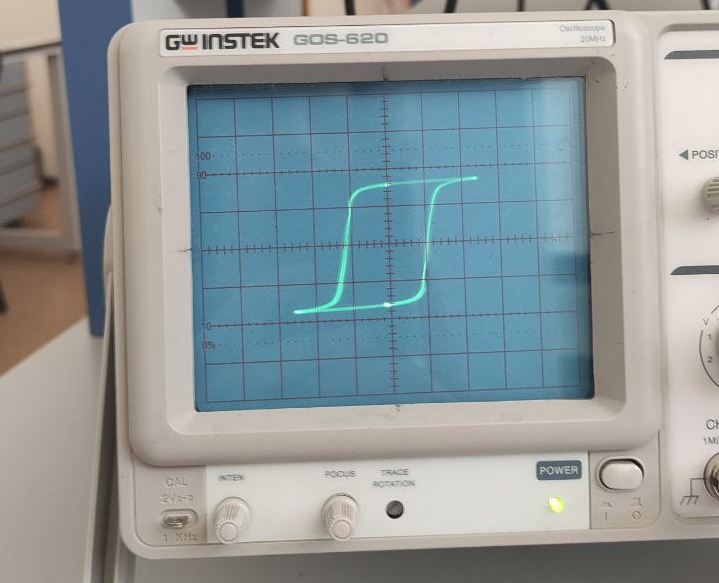
\includegraphics[width=0.5\textwidth]{Graphics/Gistr_perm.jpg}}
        \caption{График 1. Предельная петля гистерезиса пермаллоя}
\end{figure}

\begin{figure}[h]
        \center{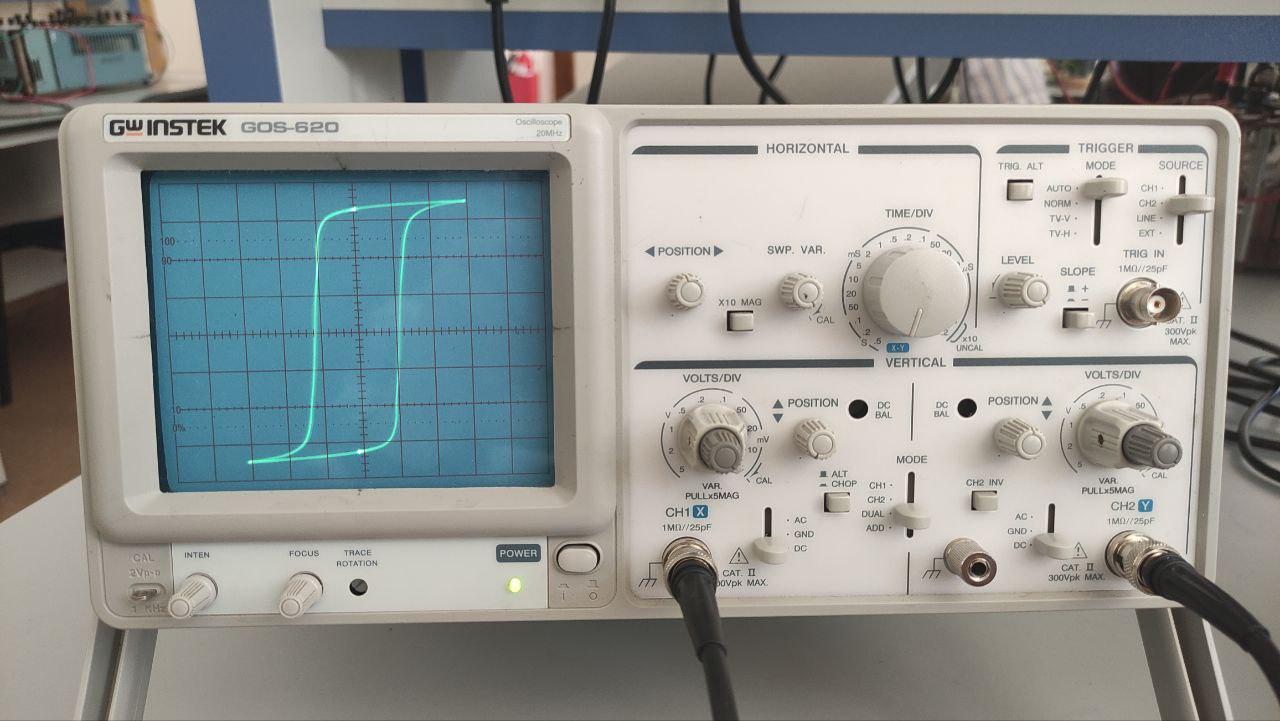
\includegraphics[width=0.5\textwidth]{Graphics/Gistr_ferrit.jpg}}
        \caption{График 2. Предельная петля гистерезиса феррита}
\end{figure}

\begin{figure}[h]
        \center{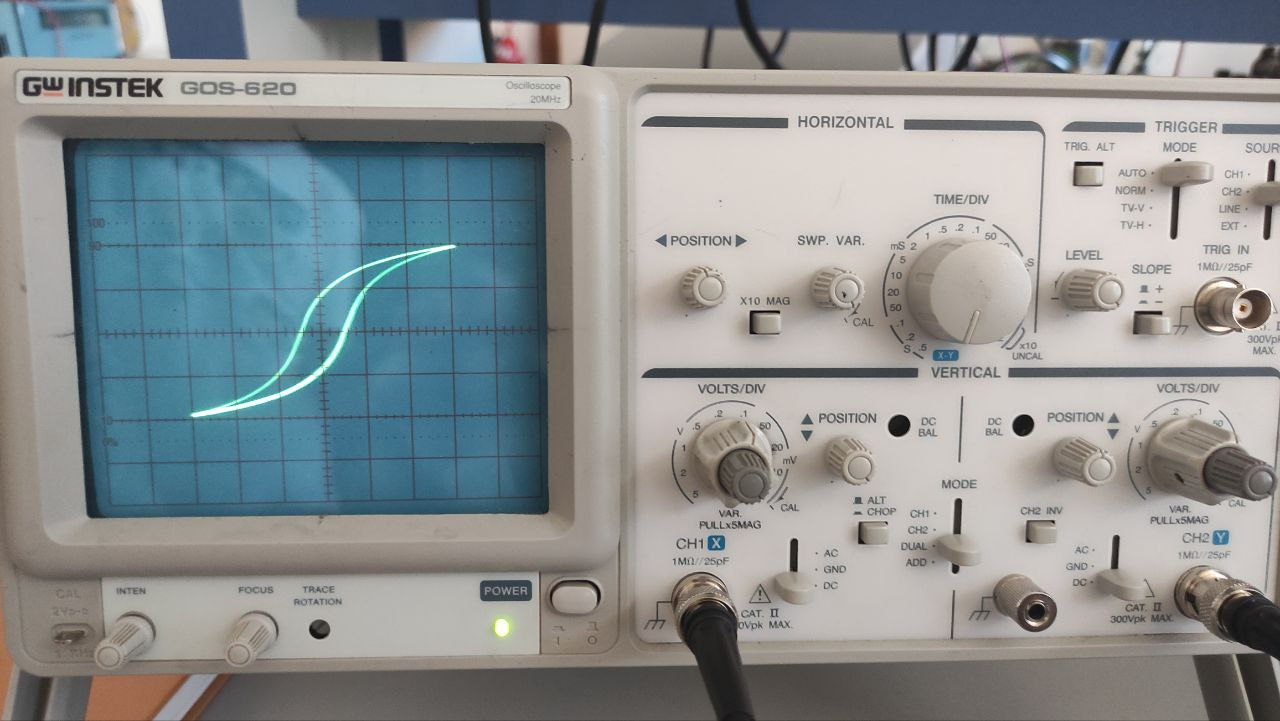
\includegraphics[width=0.5\textwidth]{Graphics/Gistr_krem_zheleza.jpg}}
        \caption{График 3. Предельная петля гистерезиса кремнистого железа}
\end{figure}
\clearpage
\item Плавное уменьшение тока и петли гистерезиса.

\begin{table}[h!]
    \centering
    \begin{tabular}{|l|c|c|c|c|c|c|c|}
        \hline
        $H,\ \text{А/м}$ & 50{,}0 & 33{,}3 & 30{,}6 & 27{,}8 & 27{,}8 & 25{,}0 & 22{,}2 \\ \hline
        $B,\ \text{Тл}$ & 0{,}337 & 0{,}295 & 0{,}232 & 0{,}189 & 0{,}126 & 0{,}074 & 0{,}021 \\ \hline
    \end{tabular}
    \caption{Таблица 6. Координаты точек кривой намагничивания для пермаллоя.}
    \label{tab:perm_points}
\end{table}

\begin{table}[h!]
    \centering
    \begin{tabular}{|l|c|c|c|c|}
        \hline
        $H,\ \text{А/м}$ & 37{,}3 & 28{,}0 & 13{,}1 & 11{,}2 \\ \hline
        $B,\ \text{Тл}$ & 0{,}200 & 0{,}160 & 0{,}027 & 0{,}013 \\ \hline
    \end{tabular}
    \caption{Таблица 7. Координаты точек кривой намагничивания для феррита.}
    \label{tab:ferrite_points}
\end{table}

\begin{table}[h!]
    \centering
    \begin{tabular}{|l|c|c|c|c|c|c|c|}
        \hline
        $H,\ \text{А/м}$ & 400{,}0 & 293{,}3 & 240{,}0 & 186{,}7 & 120{,}0 & 80{,}0 & 40{,}0 \\ \hline
        $B,\ \text{Тл}$ & 0{,}833 & 0{,}708 & 0{,}667 & 0{,}583 & 0{,}417 & 0{,}333 & 0{,}167 \\ \hline
    \end{tabular}
    \caption{Таблица 8. Координаты точек кривой намагничивания для кремнистого железа.}
    \label{tab:si_fe_points}
\end{table}

По этим данным построим кривые намагничивания и по ним найдем дифференциальные магнитные проницаемости $\mu_{\text{диф}} = \frac{1}{\mu_0} \frac{dB}{dH}$

\begin{figure}[h]
        \center{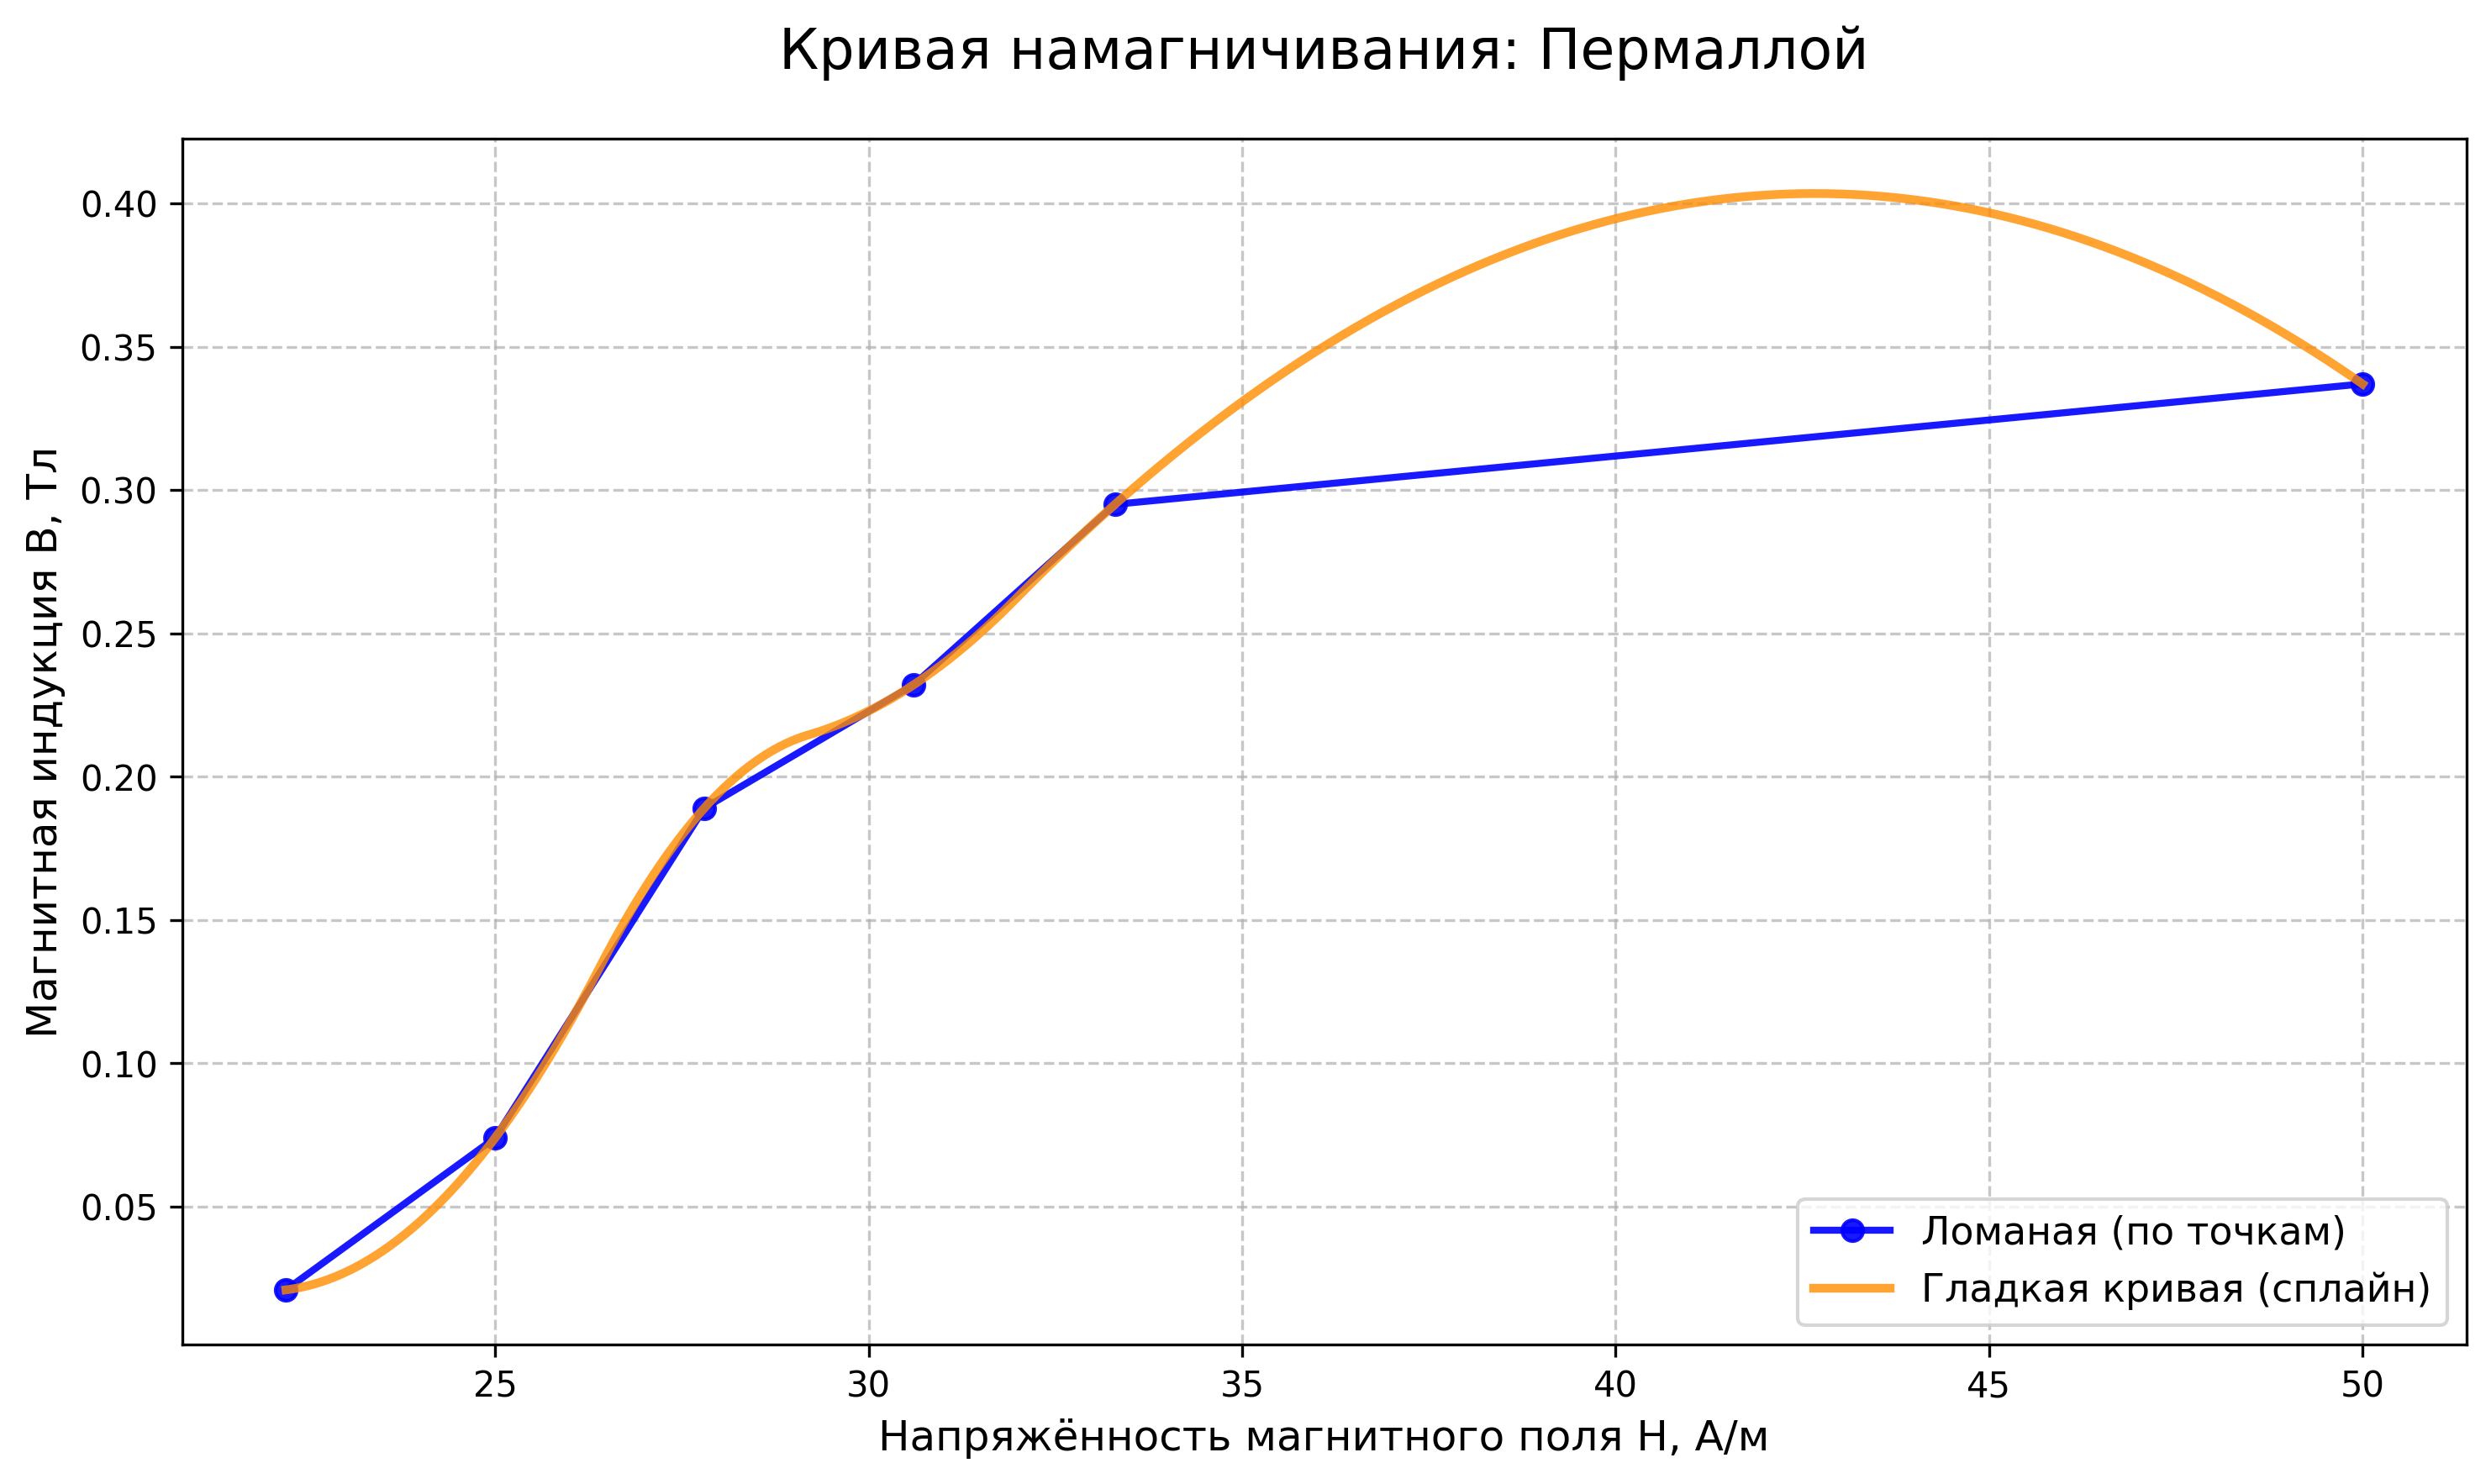
\includegraphics[width=0.7\textwidth]{Graphics/Пермаллой_B_H.png}}
        \caption{График 4. кривая намагничивания пермаллоя}
\end{figure}

\begin{figure}[h]
        \center{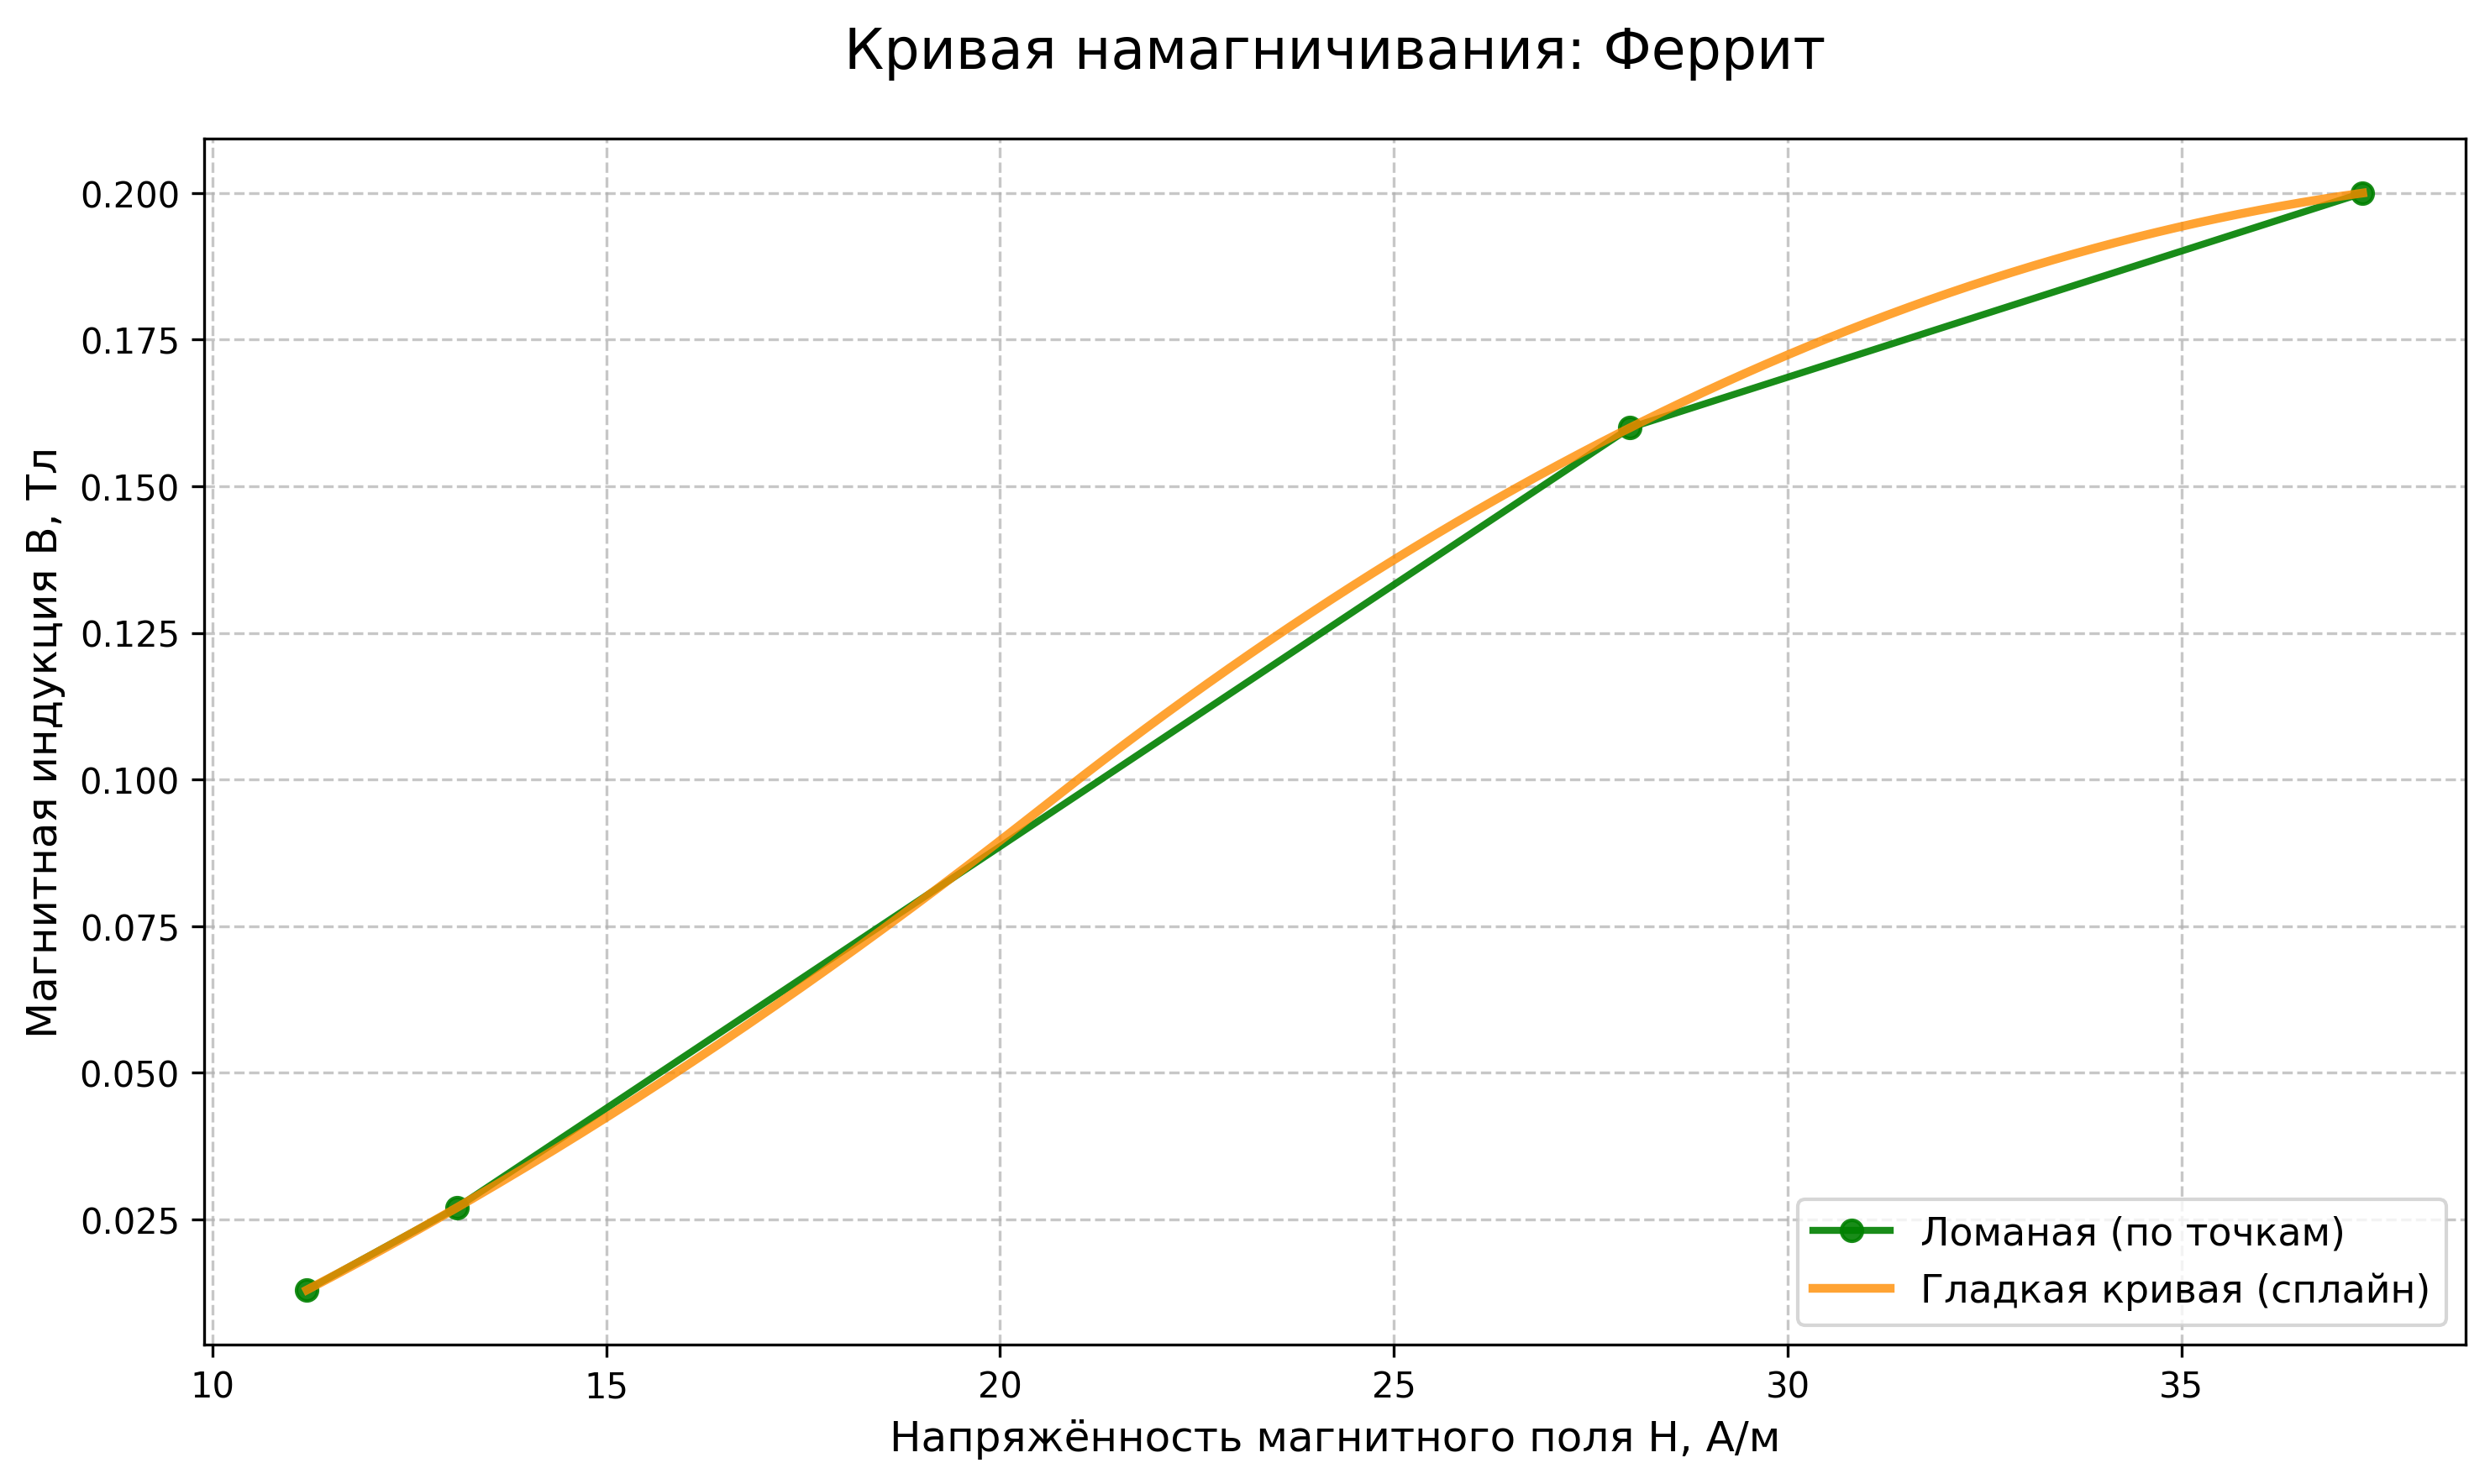
\includegraphics[width=0.7\textwidth]{Graphics/Феррит_B_H.png}}
        \caption{График 5. кривая намагничивания феррита}
\end{figure}

\begin{figure}[h]
        \center{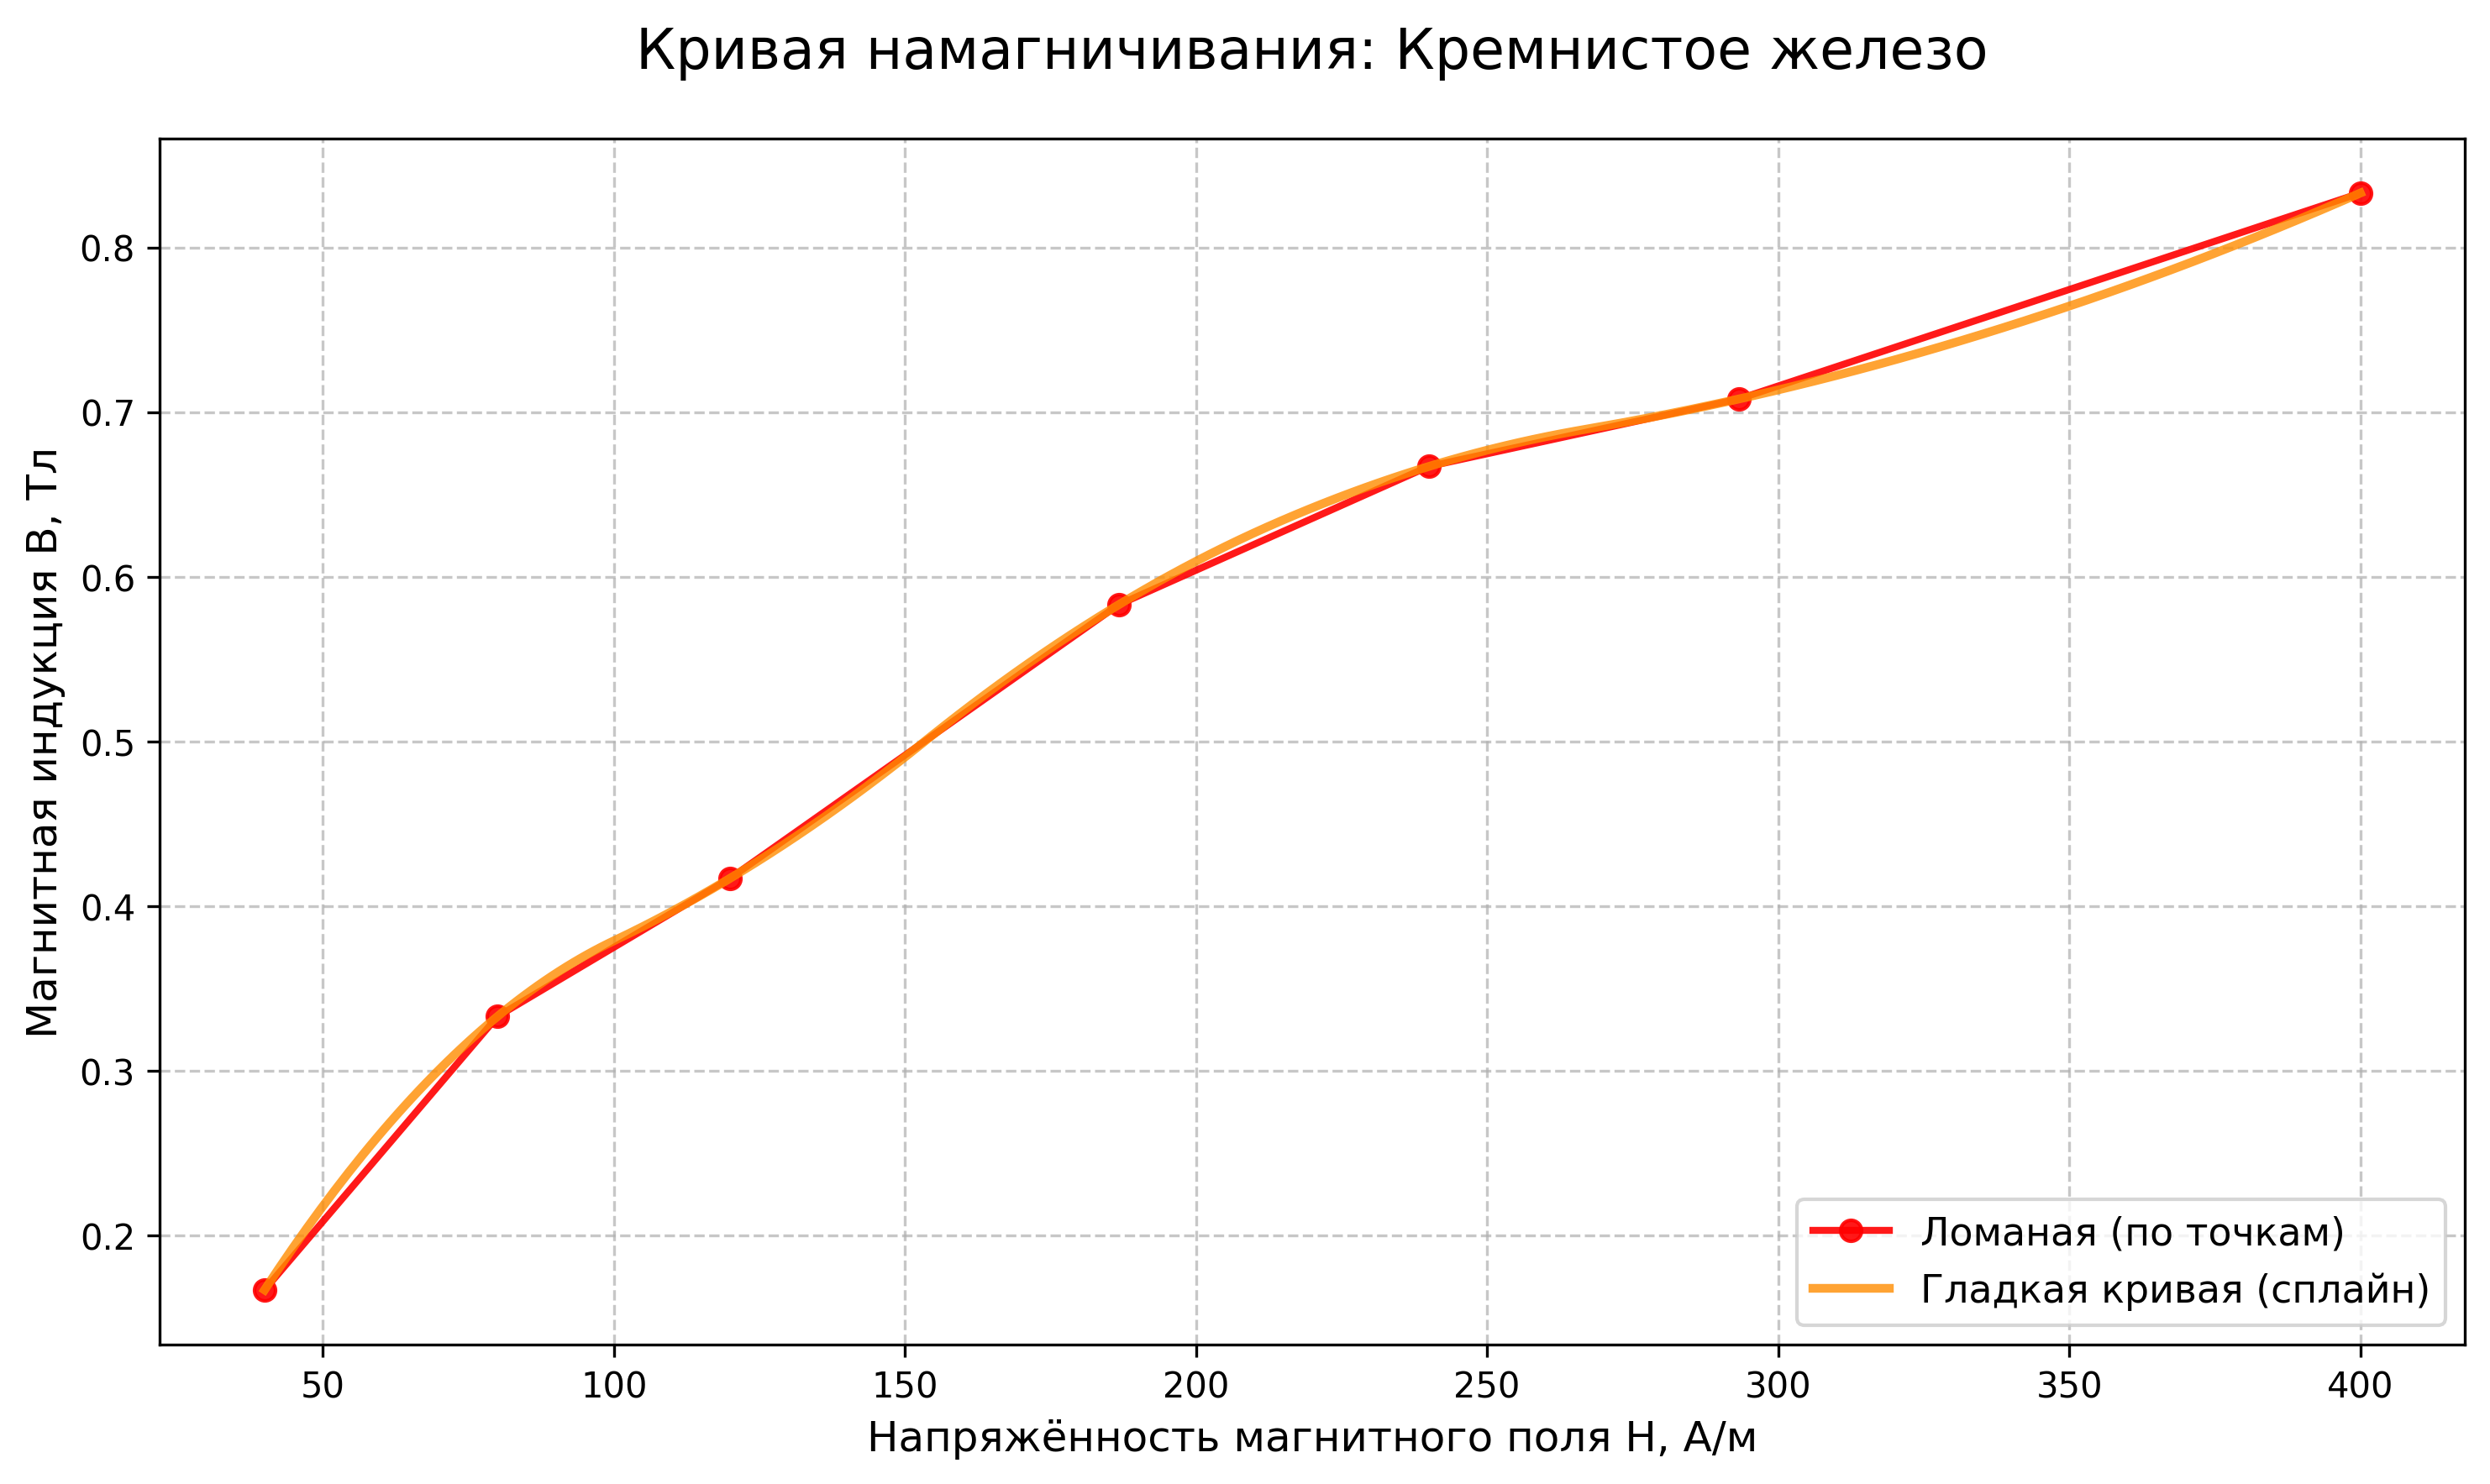
\includegraphics[width=0.7\textwidth]{Graphics/Кремнистое_железо_B_H.png}}
        \caption{График 6. кривая намагничивания кремнистого железа}
\end{figure}
\end{enumerate}
\clearpage
\section{Результаты и обсуждения}

В данной работе мы пронаблюдали за гистерезисами 3-х материалов. Вычислили предельные параметры, коэрцитивное поле и остаточную индукцию. Построили графики начальных кривых намагничивания и по ним вычислили начальные и максимальные дифференциальные магнитные проницаемости. 

\begin{table}[h!]
    \centering
    \begin{tabular}{|l|c|c|c|c|}
        \hline
        Материал & $H_c,\ \text{А/м}$ & $B_s,\ \text{Тл}$ & $\mu_{\text{диф}}^{\text{нач}}$ & $\mu_{\text{диф}}^{\text{max}}$ \\ \hline
        Пермаллой НП50 (эксп) & $27{,}8 \pm 0{,}5$ & $0{,}337 \pm 0{,}008$ & 15062{,}9 & 23873{,}2 \\ \hline
        Пермаллой 45 (табл) & 5{,}6 & 1{,}6 & 1200 & 3500 \\ \hline
        Феррит НН1000 (эксп) & $13{,}1 \pm 0{,}4$ & $0{,}200 \pm 0{,}007$ & 5863{,}6 & 6003{,}8 \\ \hline
        Феррит Ni-Zn (табл) & 16--1600 & 0{,}1--0{,}4 & 10--2000 & --- \\ \hline
        Кремнистое железо (эксп) & $66{,}7 \pm 0{,}8$ & $0{,}833 \pm 0{,}019$ & 3302{,}5 & 3302{,}5 \\ \hline
        Кремнистое железо 96Fe-4Si (табл) & 40 & 1{,}95 & 500 & 7000 \\ \hline
        Кремнистое железо 97Fe-3Si (табл) & 12 & 2{,}01 & 9000 & 40000 \\ \hline
    \end{tabular}
    \caption{Таблица. Сравнение экспериментальных и табличных значений магнитных параметров с корректно округлёнными погрешностями.}
    \label{tab:compare_with_errors_fixed}
\end{table}

Как мы видим, значения очень сильно отличаются. Ближе всего к табличным значениям оказался феррит. Расхождения связаны с множеством факторов: разный химический состав, неточность метода и измерений, геометрические особенности образцов.

\section{Выводы}
В данной работе мы изучили петли гистерезиса различных ферромагнитных торроидов: пермаллой, феррит, кремнистое железо. Построили графики, рассчитали магнитные параметры.


\end{document}